\chapter{Introduction}\label{ch:intro}

%%% Big Data intro

In recent years there has been a concerted effort to apply computer vision techniques to challenging problems which can have a positive societal impact. A highly important area where computer vision can help is conservation \cite{weinstein_computer_2018}. One of the main goals of conservation research is to monitor animal populations in their distribution area, undertaking abundance estimates to inform policy change. This is most commonly performed using capture-recapture surveys where researchers identify the presence of individuals and estimate abundance of animals in an area to produce population estimates \cite{constantine_abundance_2012, bigg_assessment_1982, sharpe_indian_2019, van_bressem_visual_2018, arso_civil_changing_2019, cheney_long-term_2014}. These surveys can be classified as invasive where animals are physically trapped, tagged, and released \cite{norris_tagging_1970, hobbs_bowhead_1982, andrews_best_2019}, or non-invasive where monitoring is performed passively such as via the collection of vast numbers of images \cite{vanbressem_visual_2018, urian_recommendations_2015, reisser_photographic_2008, langtimm_survival_2004, holmberg_estimating_2009}.

Photo-id is one of the main non-invasive capture-recapture methods utilised by cetacean (dolphin, porpoises, and whales) researchers \cite{hammond_individual_1990, evans_monitoring_2004}. Surveys are usually undertaken from vessels at sea, although monitoring from coastlines or aircraft may also be utilised \cite{payne_long_1986, forney_seasonal_1998, wursig_methods_1990}. The methodology is employed for the monitoring of multiple cetacean species, with proven use cases in a range of studies \cite{sharpe_indian_2019, miragliuolo_rissos_2004, feyrer_origin_2021, bigg_assessment_1982}. Outside of cetaceans, photo-id has found further use in study of other marine life \cite{holmberg_estimating_2009, reisser_photographic_2008} and terrestrial species \cite{goswami_application_2007, clapham_automated_2020}.

All capture-recapture methodologies rely on the target species having some form of individually identifiable markings. Depending on the species, different parts of the body are the primary identifying feature; for dolphins this is usually the dorsal fin as this body part is most likely to be visible above the waterline \cite{sharpe_indian_2019, baird_population_2009}. During photo-id surveys, researchers often focus on long lasting stable markers such as dorsal fin shape, notches, scarring, and pigmentation \cite{wursig_photographic_1977, lockyer_observations_1990, mann_cetacean_2000}. These markings can be difficult to capture in detail due to the free roaming nature of the animals causing high variances in angles of approach, direction of travel, distance from camera, and surfacing elevation. This is exacerbated when dealing with cetacean species that travel in pods, making it difficult to distinguish the individuals present.

Marine photo-id can be extremely labour and cost intensive compared to on-land surveys, which rely on the use of camera traps placed in stationary locations to capture images when they detect movement. This setup is not possible at sea due to a lack of stationary objects to attach devices to and rapid movement in the observed scene due to waves causing the camera to trigger -- producing a high false positive rate. 

Upon survey completion, photo-id data must be analysed and individuals identified to produce a catalogue. Images collected during surveys are large in size and contain significant amounts of background noise. Historically, curation of this data has been a manual process that often takes longer than the entire data collection period \cite{tyson_moore_rise_2022}, further increasing labour and costs. As such, any techniques to speed up the cataloguing process would be welcomed both by researchers and their funding bodies, affording more time to work on the application of data, for example to inform mitigation and policy change, rather than curation. 

This thesis details a system for fully automatic catalogue matching based on unprocessed photo-id imagery. This is achieved through a pipeline of trained computer vision models and robust post-processing techniques capable of automatic fin detection and most likely catalogue matching based on latent space similarity, a visualisation of which can be seen in Figure \ref{fig:pipeline}. 

\begin{figure}[b]
	\begin{center}
		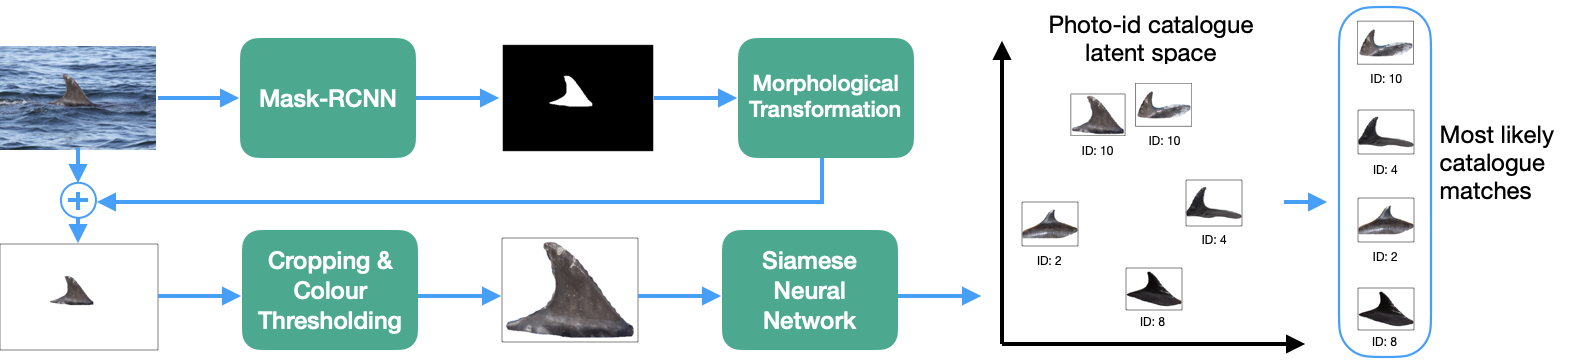
\includegraphics[width=\linewidth]{Chapter1/figs/pipeline_compact.png}
	\end{center}
	\caption{A high level overview of data flow through the proposed system.}
	\label{fig:pipeline}
\end{figure}

As photo-id surveys are not guaranteed to capture all individuals in a given geographic area, naive approaches such as training a simple image classifier on existing catalogue examples would not suffice as they are incapable of flagging previously uncatalogued individuals. Images are passed through a Mask R-CNN \cite{he_mask_2017} dorsal fin detector, removing the need for manual data pre-processing. Detections are then post-processed ready for fine-grained, few-shot catalogue matching utilising a Siamese Neural Network trained using triplet loss \cite{schroff_facenet_2015} and online semi-hard triplet mining to create a latent space based on the provided catalogue. Matches are obtained using the Euclidean distances between an input and class prototypes stored in the latent space, allowing for the flagging of potentially uncatalogued individuals to the researcher.

\section{Research Aim and Contributions}\label{ch:intro,sec:AimsAndContributions}

The high level aim of this thesis is to:

\begin{flushleft}
	\textbf{Design, implement, and evaluate a system for fully automatic catalogue matching based on unprocessed photo-id fieldwork imagery.}
	\bigbreak\noindent Implicit in this aim are a number of research questions:
\end{flushleft}

\begin{enumerate}
	\item Is it possible to remove or greatly reduce the need for manual pre-processing of photo-id data in a fully automated way through the use of coarse-grained detection?
	\item Can post-processing of detections be performed in such a way as to both reject likely false positives and remove noise whilst retaining identifiable markings?
	\item ls it possible to perform highly accurate most likely photo-id catalogue matching based on extreme fine-grained information, even when operating on few-shot data?
	\item How generalisable are the above concepts to changes in species of interest and spatio-temporal shifts?
\end{enumerate}

\noindent To answer these questions and thereby address its aim, this thesis presents the following contributions:

\begin{enumerate}
	\item A detailed survey on the current state of the art in applied computer vision for cetacean conservation. Existing photo-id aides are described and evaluated, providing a framework to understand their shortcomings. This is presented in Chapter \ref{ch:Background}. 
	\item A highly accurate Mask R-CNN \cite{he_mask_2017} based coarse-grained cetacean detector, capable of generating pixel-wise mask predictions from above water photo-id survey imagery. The detector is invariant to both the extreme variation in RoI shape inherently present due to the free roaming nature of cetaceans, and the large amount of noise generated as a result of operating in marine environments.  This is presented in Chapter \ref{ch:cetDet}.
	\item A framework for the robust post-processing of predicted RoIs produced by the cetacean detector with the aim of preventing false-positives from moving downstream. Predictions are automatically cleaned, allowing for removal of noise and enhancement of the prominence of individually identifying markings and removing the need for manual data pre-processing. This is presented in Chapter \ref{ch:cetDet}.
	\item An open-source dataset, called \textit{The Northumberland Dolphin Dataset 2020}, for use in the evaluation of photo-id aides. Curated from imagery collected during fieldwork undertaken off the coast of Northumberland, UK, this dataset allows for the generalisability of the aforementioned coarse-grained cetacean detector to be tested, examining its robustness to changes in species of interest and spatio-temporal shifts. The dataset is released publicly to aid in the development of future photo-id aides, providing open-source data to a research area where this is not yet commonplace. This is presented in Chapter \ref{ch:NDD}.
	\item A Siamese Neural Network (SNN) based computer vision model capable of fine-grained, few-shot catalogue matching using the post-processed detections passed downstream by previous system components. Inputs to the model are embedded into a latent space to generate a list of most likely catalogue matches using class prototypes and Euclidean distance measurements, which also allows the model to flag potentially previously uncatalogued individuals to the user. Implementation work is presented in Chapter \ref{ch:ID}, with generalisability evaluation using a second real-life photo-id catalogue presented in Chapter \ref{ch:SNNEvaluation}.
\end{enumerate}

\section{Thesis Structure}\label{ch:intro,sec:Structure}

The structure of this thesis is as follows:

\begin{description}
	\item[Chapter \ref{ch:intro}] provides the motivation for the work undertaken in this thesis, and highlights its main contributions. An overview of the peer-reviewed publications produced as a result of work undertaken in fulfilment of this thesis is also presented.
	
	\item[Chapter \ref{ch:Background}] presents the required background knowledge for understanding the work presented in future chapters. An introduction to both photo-id and deep learning is provided, alongside a discussion of key computer vision concepts and their recent use in conservation. Existing photo-id aids are also examined.
	
	\item[Chapter \ref{ch:cetDet}] outlines the approach adopted to create a computer vision model capable of coarse-grained cetacean detection in noisy, above water photo-id fieldwork imagery. Initial model testing is discussed, including the use of transfer learning, data augmentation, and hyperparameter tuning via a grid search. Next, the use of post-processing techniques to reduce the passing of false-positives downstream through the system pipeline is explored. 
	
	\item[Chapter \ref{ch:NDD}] describes the data collection fieldwork undertaken off the coast of Northumberland, UK, during Summer 2019. The curation of this data into a useable dataset for the training of computer vision models is explained. The robustness of work outlined in Chapter \ref{ch:cetDet} is evaluated using the dataset. 
	
	\item[Chapter \ref{ch:ID}] outlines the possible approaches available to the task of automated fine-grained, few-shot most likely catalogue matching. The implementation of the chosen approach is examined in detail, including model training, evaluation metrics, and hyperparameter tuning via Bayesian optimisation. The use of uncatalogued individual thresholding is examined using generated class prototypes, Euclidean distance measurement, and the K-Nearest Neighbours algorithm over the model's latent space. 
	
	\item[Chapter \ref{ch:SNNEvaluation}] evaluates the chosen approach to most likely catalogue matching outlined in Chapter \ref{ch:ID}. Various data perturbations and their effect on model performance are examined, as well as a robustness evaluation using a second real-life photo-id catalogue to explore the generalisability of the model, the previously determined uncatalogued individual thresholds, and the effect of species of interest and spatio-temporal changes.
	
	\item[Chapter \ref{ch:Conclusion}] summarises the conclusions of the work presented in this thesis and explores avenues for future work in the area.  
	 
\end{description}

\section{Related Publications}\label{ch:intro,relatedPublications}

The work outlined in this thesis has led to the publication of the following peer-reviewed papers:

\begin{description}
	\item[\cite{trotter_northumberland_2019}] Trotter, C., Atkinson, G., Sharpe, M., McGough, A.S., Wright, N. and Berggren, P., 2019. The Northumberland Dolphin Dataset: A Multimedia Individual Cetacean Dataset for Fine-Grained Categorisation. In \textit{The 6\textsuperscript{th} Workshop on Fine-Grained Visual Categorization, CVPR 2019}. Available: \href{https://doi.org/10.48550/arXiv.1908.02669}{doi.org/10.48550/arXiv.1908.02669}.
	
	\item[\cite{trotter_ndd20_2020}] Trotter, C., Atkinson, G., Sharpe, M., Richardson, K., McGough, A.S., Wright, N., Burville, B. and Berggren, P., 2020. NDD20: A large-scale few-shot dolphin dataset for coarse and fine-grained categorisation. In \textit{The 7\textsuperscript{th} Workshop on Fine-Grained Visual Categorization, CVPR 2020}. Available: \href{https://doi.org/10.48550/arXiv.2005.13359}{doi.org/10.48550/arXiv.2005.13359}.
\end{description}

\newpage

\noindent The following work into the application of computer vision to conservation was produced during, but does not form a part of, this thesis:

\begin{description}
	\item[\cite{curry_application_2021}] Curry, R., Trotter, C. and McGough, A.S., 2021, December. Application of deep learning to camera trap data for ecologists in planning/engineering – Can captivity imagery train a model which generalises to the wild?. In \textit{2021 IEEE International Conference on Big Data (Big Data)} (pp. 4011-4020). IEEE. Available: \href{	https://doi.org/10.1109/BigData52589.2021.9671661}{doi.org/10.1109/BigData52589.2021.9671661}.
\end{description}



%%%%%%%%%%%%%%%%%%%%%%%%%%%%%%%%%%
% All nomenclature here for ease
\nomenclature[z-CNN]{CNN}{Convolutional Neural Networks}
\nomenclature[z-CPU]{CPU}{Central Processing Unit}
\nomenclature[z-GPU]{GPU}{Graphical Processing Unit}
\nomenclature[z-SGD]{SGD}{Stochastic Gradient Descent}
\nomenclature[z-SGDR]{SGDR}{Stochastic Gradient Descent with Restarts}
\nomenclature[z-ReLU]{ReLU}{Rectified Linear Unit}
\nomenclature[z-FCN]{FCN}{Fully Convolutional Network}
\nomenclature[z-RPN]{RPN}{Region Proposal Network}
\nomenclature[z-VM]{VM}{Virtual Machine}
\nomenclature[z-MCZ]{MCZ}{Marine Conservation Zone}
\nomenclature[z-RIB]{RIB}{Rigid Inflatable Boat}
\nomenclature[z-NDD20]{NDD20}{Northumberland Dolphin Dataset 2020}
\nomenclature[z-SMRU]{SMRU}{Sea Mammal Research Unit}
\nomenclature[z-PCA]{PCA}{Principle Component Analysis}
\nomenclature[z-SURF]{SURF}{Speeded-Up Robust Features}
\nomenclature[z-SIFT]{SIFT}{Scale-Invariant Feature Transform}
\nomenclature[z-TPE]{TPE}{Tree-structured Parzen Estimator}	
\nomenclature[z-KNN]{KNN}{K-Nearest Neighbours}
\nomenclature[z-SDRP]{SDRP}{Sarasota Dolphin Research Program}
\nomenclature[z-RoI]{RoI}{Region of Interest}
\nomenclature[z-mAP]{mAP}{Mean Average Precision}
\nomenclature[z-IOU]{IOU}{Intersection Over Union}
\nomenclature[z-NLP]{NLP}{Natural Language Processing}
\nomenclature[z-ViT]{ViT}{Vision Transformer}
\nomenclature[z-GUI]{GUI}{Graphical User Interface}
\nomenclature[z-UAV]{UAV}{Unmanned Aerial Vehicle}
\nomenclature[z-MLOps]{MLOps}{Machine Learning Operations}
\nomenclature[z-RPN]{RPN}{Region Proposal Network}